\pagenumbering{arabic}

\chapter{Definitions and Properties}

\textbf{Computer/Information security:}
\\The protection \textit{afforded} to an automated information system in order to attain the applicable objectives of \textit{preserving} the \underline{Confidentiality, Integrity, and the Availability} of information systems resources. (refers to ACI, not to the computer/device/hardware) (preserving not creating)(not possible perfect security)
\\\textbf{Cyberspace:}
\\Domain characterized by the use of electronics and the electromagnetic spectrum to store, modify and exchange data via networker systems and \underline{associated physical infrastructures}. \\\textit{NB: From IT to cyberspace, same domain and still with electronics but even with physical systems.}
\\\textbf{Cybersecurity:}
\\Is the art of \underline{protecting} networks, devices and data from \underline{unauthorized} (access not authorized to a device) or \underline{criminal} use and the practice of ensuring integrity, availability and confidentiality. Cybersecurity is the practice of protecting systems, networks, and programs from digital attacks… Prevention of damage to, protection of, and restoration of computer, electronic communications systems, electronic communications services, wire communication, and electronic communication, including information contained therein, to ensure its availability, integrity, authentication, confidentiality and non-repudiation. Cybersecurity is the practice of protecting critical systems and sensitive information from digital attacks. Also known as information technology (IT) security, its measures are designed to combat threats against networked systems and applications, whether those originate from inside or outside of an organization.
Cybersecurity domains are several, education, tech, IoT, matter of governance…
\\\textbf{Trust:}
Is the acceptance of the truth of a statement without evidence or investigation; it is blind faith or wishful thinking if you will.
\\\textbf{Trusted:}
\\Able to be depended on → you cannot verify.
\\\textbf{Trustworthy:}
\\Worth to be trusted → upon verification.
\\\textbf{Safety:}
\\The condition of not being in danger or of not being dangerous: For your safety, keep your seat belt securely fastened.
\\\textbf{Security:}
\\Protection of a person, building, organization, or country against
threats such as crime or attacks.
\\\textbf{Dependability:}
\\The property of a computer system such that reliance can justifiably be placed on the service it delivers. Behaving as expected.
\\\textbf{Resilience:}
\\The ability to operate correctly (even with reduced functionality) or restore a safe state while the system is compromised or after an attack.
\\\\Usage is important, with Cyber-Physical Systems usage of the system is also a crucial issue besides traditional security properties of its information (Safety issues) and the solution must be a combination of analogue and digital world.
\\  \indent Es: In a classical IT system, the reaction to an access control violation is to stop \indent the access to the requested resource. In a CPS that could have dangerous collateral \indent effects. Imagine the braking system of a modern car…
\\\textit{PS: The course focuses on digital networks and systems, thus on the traditional CIA and related properties.}
\\\\We are moving away from cybersecurity to land on cyber resilience.
\\\textit{NB: things are very complicated so it’s difficult to protect $\Rightarrow$ from cybersec to resilience $\Rightarrow$ the goal it’s not anymore to prevent attack (system will be attacked) so you try to regain safe status.} 
\\But wait, wasn’t computer security about creating security/cracking security/hacking security? No. Rather, it is about \underline{preserving} security.
What does this mean? That you can only preserve something that you already have and that security technologies do not build security properties. They “merely” make sure that the security properties that are already there are maintained.
We need to understand two concepts: what is there to be preserved and what is the “built-in” security that needs to be preserved.
\\\textit{NB: What is it that computers do? $\Rightarrow$  Operate over information $\Rightarrow$ Information is everything that operates and is operated by a computer (computer program, temporary functions, variables, excel file, picture...)}
All a computer system is about is information. So preserving what? Properties of information.
At the bare minimum, any “piece of information” is only useful if it can be reached and read and is correct. $\Rightarrow$ These can be seen as “properties” of information.
\\Computer security is about preserving these properties:
\begin{itemize}
\item Confidentiality$\Rightarrow$ Assure that a piece of info can be read only by those who are authorized to read it (only you can read what you need to read);
\item Integrity$\Rightarrow$ Prevent unauthorized modification of information (prevent unauthorized writing). While data integrity, integrity synonymous for external consistency.(within the bounding of digital signals(info giuste da me ma devono anche arrivare giuste(external consistency)));
\item Availability$\Rightarrow$ Assure that a piece of information can be reached when needed.
\end{itemize}
\textit{NB: This is known as the CIA triad that are the “core” security properties of a piece of information. On top of this, one can build additional properties like Accountability (The ability to know with certainty who/what operated on a piece of information), Non-repudiation (The entity that acted on the information can not “repudiate” his/her/its action), Authentication (alone has no meaning, it depends of the subject:
\begin{itemize}
    \item \textbf{User authentication:} The ability to prove that a person is who she claims to be;
    \item \textbf{Message/Data authentication:} assurance that the message has been signed with a particular key;
    \item \textbf{Sender authentication:} assurance that the message has been sent by a party (IP address, server, computer, process, etc.)) etc…
\end{itemize}
}

But who can act upon information?
\\Humans are not the only “users” of information, the human user of the system avertedly or un-avertedly modifies information. A system/software/module/thread can act on the whole system (or another system) on behalf of a human user $\Rightarrow$ “Delegation” is the mechanism by which, for example, software threads are spawned (E.g., with the privileges of the entity that spawned it). While a human user may or may not know what they do a “surrogate” does not. There is no notion of “avertedly” or “un-avertedly”.
Computer systems do not know what they are doing. They can only execute instructions (information) to operate over some other information. Systems can only be instructed to preserve the security properties of that information by means of some mechanism(es Confidentiality $\Rightarrow$ crypto, Integrity $\Rightarrow$ secure hardware, Availability $\Rightarrow$ redundancy).
\\\\Esempietti carini che ha fatto: CBC $\Rightarrow$ sai che prendi roba e la butti nel blocco, quando esce la unisci con altra e la butti nel prossimo blocco… problema se qualcuno cambia ste cose (change bits) $\Rightarrow$ attacks because pc doesn’t understand that something goes wrong, a human yes but computer no, it’s a little bit stupid, so attacker actions produces an invalid value and, because the missing sanity check, there is an attack.
\\\\Altro esempietto cutie: Zero trust (è legato alla roba del TCB $\Rightarrow$ Trusting Computing Base che vedrai dopo, $\Rightarrow$ Combination of hardware, firmware, and software that can breach your security policy).
Practically I need a secure/trusting component to build a system, but what about zero-trust architectures?
\begin{figure}[h]
    \centering
    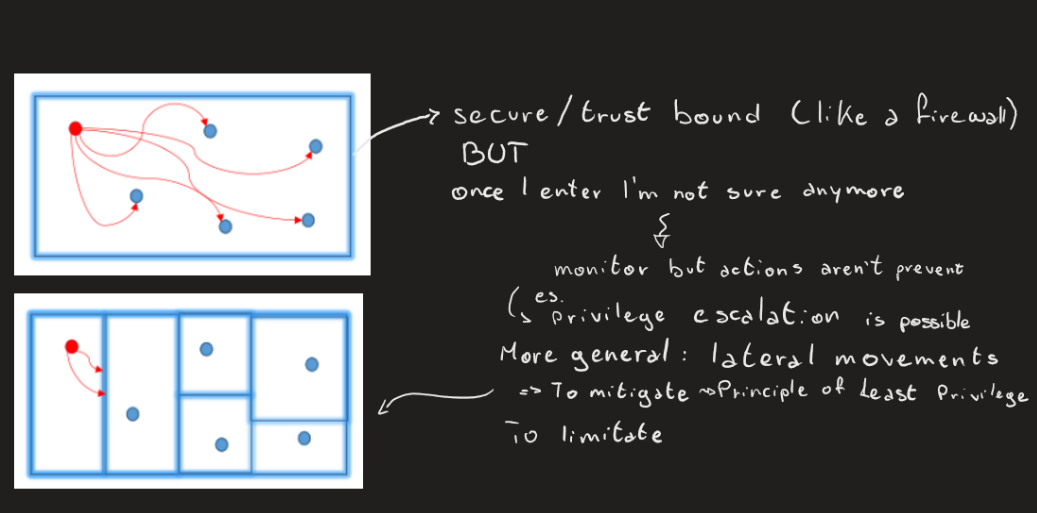
\includegraphics[scale=0.5]{Figures/ZeroTrust.png}
    \caption{Zero Trust}
\end{figure}
\\Trust in information security (more formally)
\begin{itemize}
    \item Ken Thompson, 1983 ACM Turing Award Lecture
    \item “Reflections on Trusting Trust” is a mandatory reading, http://dl.acm.org/citation.cfm?id=358210
    \item Suggested reading:
    \item Bruce Schneier, ”Attack trees”, Dr. Dobb's Journal, December 1999.
\end{itemize}
So, what software/system can one trust?
\\Imagine an authentication mechanism $\Rightarrow$ User inputs username, User inputs password, User presses enter, User has access to desktop…There are a lot of trust assumptions here!
The user trusts the authentication mechanism. But what really happened? Did the authentication sw do the actual match? Will it only grant access if it matches your credentials? Did it send your credentials to a third party? Did it use your credentials to read and copy your data?
How do you increase your level of trust in the software? You can look at the source code, but is this enough?
\\\textbf{Example:}

\begin{figure}[h]
    \centering
    \begin{subfigure}[b]{0.4\textwidth}
        \centering
        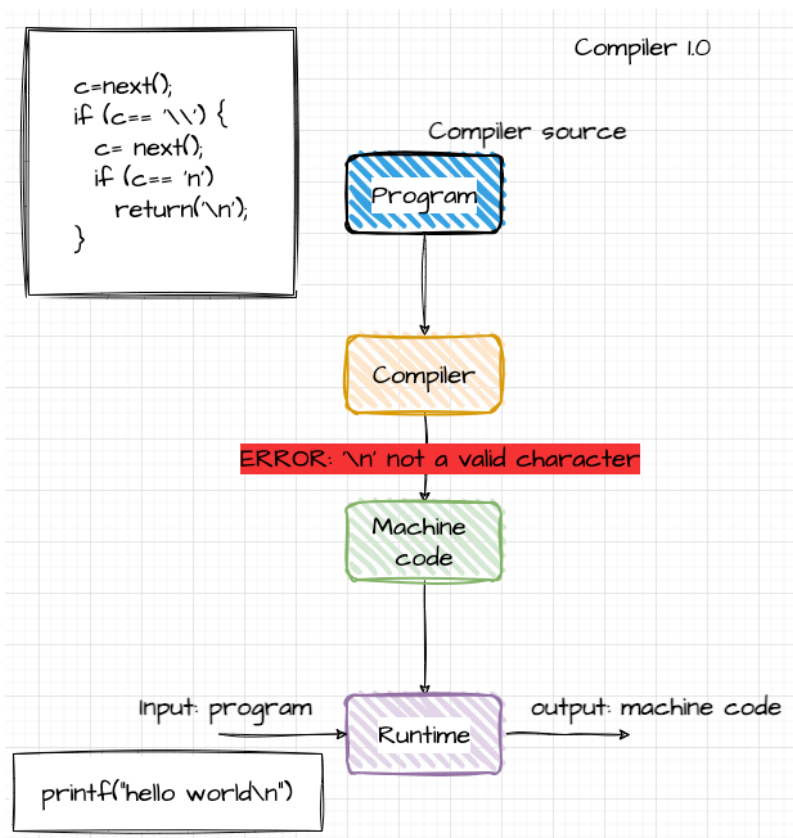
\includegraphics[width=\textwidth]{Figures/Compiler0.png}
        \caption{Compiler 1.0}
        \label{Compiler 1.0}
    \end{subfigure}
    \hfill
    \begin{subfigure}[b]{0.4\textwidth}
        \centering
        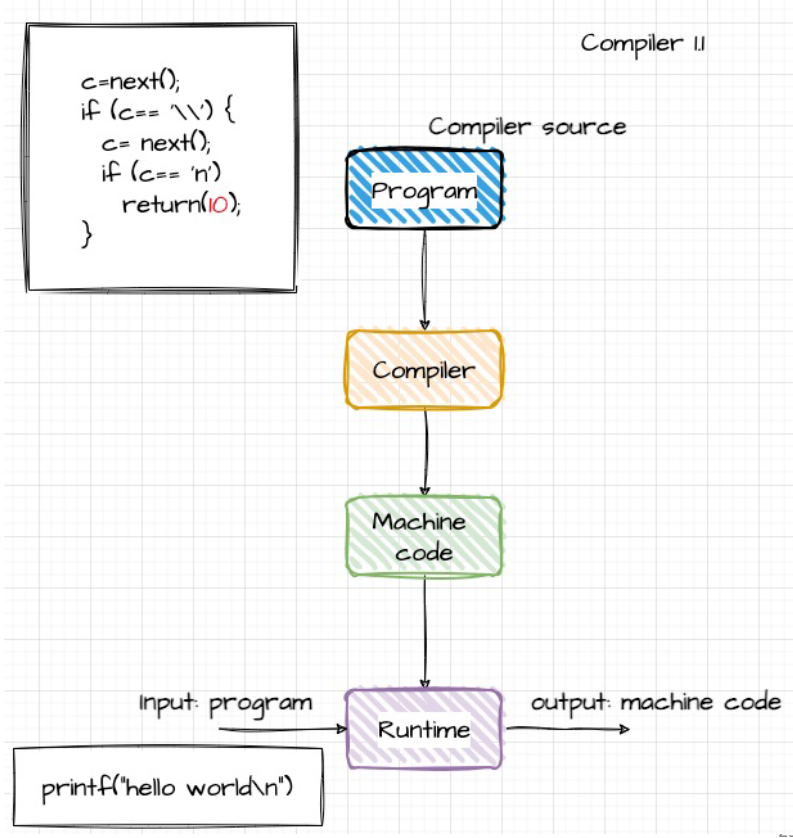
\includegraphics[width=\textwidth]{Figures/Compiler1.png}
        \caption{Compiler 1.1}
        \label{Compiler 1.1}
    \end{subfigure}
\end{figure}

What or who did really generate that software? The human being that wrote the sw source code? The compiler that compiled the sw source code? The human being that wrote the compiler that compiles the sw source code? The compiler that compiles the compiler that compiled the sw source code?...
So who do you trust?
Thompson’s view $\Rightarrow$The compiler can be modified in any way to include
code that never appears in the sw source code, and depending on how many generations passed, it won’t appear in the previous compiler versions source code either.
$\Rightarrow$ Trusting trust: You can't trust code that you did not totally create yourself. No	
amount of source-level verification or scrutiny will protect you from using untrusted code.”


Computer Security vs Network Security

A computer network is a general architecture that allows computer systems to share information remotely. Network security is based on the same exact idea of preserving the CIA properties of information, it makes for an especially interesting case.
Who can be trusted over the network? Can you trust your own system? Can you trust the communication channel? Can you trust the destination system?


CLIENT-SERVER RECAP FOR DUMMIES, TECHNICAL LOOK, ATTACK POINTS (when 2 component, spinning 2 different processes, that are not suppose to interact, are forced/needed to interact-> an attacker can create a gap/bridge-> vulnerability!) LEGACY ISSUE



ATTACK
A general attacker might infiltrate the communication in between hops, impersonate the client, modify connections/routing, be/infiltrate one of the hops or act “legally” until end of service (after which it may act maliciously)...


*Attack trees*


Attack models in network setting: outright malicious attacker

Typically, the malicious attacker aims at reading or modifying the messages (in part or fully)->That’s a confidentiality, integrity, availability problem.
In this contest, this attacker is typically called “man in the middle” or “man in the browser”. Attackers can intercept and act upon a communication between client and server, such as channel redirection, block communication entirely or spoofing the user’s identity.
An example could be injection of malicious content, in which there is a manipulation of server response, then client’s answer can also be modified by the attacker, so a connection Hijack and finally attacker injects him/herself in the communication and spoofs the victim’s identity.
NB: Formally known as the Dolev-Yao model, it applies to any entity of the network

Attack models in network setting: Honest-but-curious attacker
The goal of this attacker is to use the client’s information after correctly handling the service. Typically resides at the service level, e.g. ISP,  and implies confidentiality and possibly integrity threats.
A possible example could be where DB Server is the attacker, it provides agreed service
correctly, like answers queries with correct data. After the query is delivered to the client, the server uses the query’s information to perform user profiling.


